\renewcommand{\thesection}{\Alph{section}}
\definecolor{airforceblue}{rgb}{0.36, 0.54, 0.66}
\definecolor{ballblue}{rgb}{0.13, 0.67, 0.8}
\setcounter{figure}{0}
\renewcommand{\thefigure}{\Alph{section}.\arabic{figure}}
\appendix
\addchap{Anhang}

\newcolumntype{C}[1]{>{\centering\let\newline\\\arraybackslash\hspace{0pt}}m{#1}}

\captionsetup{list=false}

\section{Bilder}
\begin{figure}[H]
\centering
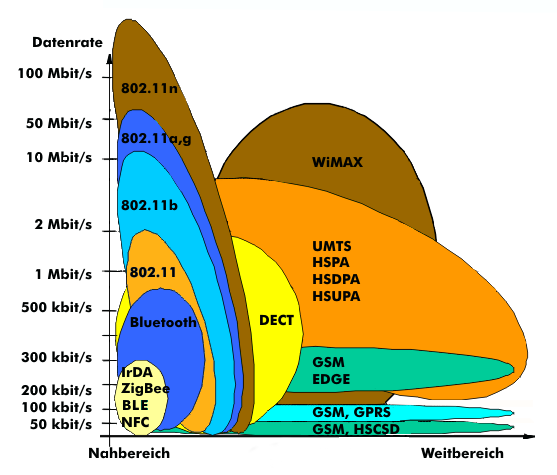
\includegraphics[scale=1]{Bilder/Funktechnologien.png} 
\caption{Überblick zu heutigen Funktechnologien \cite{FUE}}
\label{fig:FUE}
\end{figure}

\section{Tabellen}
Beispielwerte für einen Beacon-Einsatz
\begin{center}
\begin{tabular}{|c|c|C{3cm}|C{3cm}|C{3cm}|}
\hline
\rowcolor{airforceblue} \multicolumn{2}{|c|}{\textbf{Geschäftsstandort}} & \textbf{Berlin}  & \textbf{Magdeburg} & \textbf{München} \\ \hline
\multicolumn{2}{|c|}{\cellcolor{ballblue} \textbf{UUID}}    & \multicolumn{3}{c|}{U8T7V56I-4689-10U9-7G63B4GAR21M}\\ \hline
\multicolumn{2}{|c|}{\cellcolor{ballblue} \textbf{Sendestärke} }    & -12dBm   & -6dBm & 1dBm \\ \hline
\multicolumn{2}{|c|}{\cellcolor{ballblue} \textbf{Major}}    & 1  & 2 & 3\\ \hline
\cellcolor{ballblue} & \cellcolor{ballblue} \textbf{Kleidung}    & 10  & 10 & 10\\ \cline{2-5}
\cellcolor{ballblue} & \cellcolor{ballblue} \textbf{Elektronik}    & 20  & 20 & 20\\ \cline{2-5}
\cellcolor{ballblue} \multirow{-3}{*}{\textbf{Minor}}& \cellcolor{ballblue} \textbf{Küche}    & 30  & 30 & 30\\ \cline{2-5}
\hline
\end{tabular}
\end{center}

\section{App-Aufbau}
Anhang für die einzelnen App-Bestandteile.

